\documentclass[11pt]{amsbook}

\usepackage{../HBSuerDemir}

\begin{document}

 
    
	
\hPage{b2p1/206}

\begin{minipage}{.1\linewidth}
    
                           
    \section*{\underline{Particular Case:}}
 
\end{minipage}


\par
 Particular case of cylinders, cones, surfaces of revolutions 
are obtained by taking the generatix $\Gamma$ on a coordinate plane.\\ 
\par


\begin{minipage}{.1\linewidth}
    
                           
    \section{\underline{Cylinders}}
 
\end{minipage}
    
 
\par\noindent               
    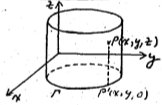
\includegraphics[ width=5 cm,height=2 cm]{b2p1-206-fig01-jpg}
    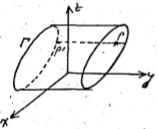
\includegraphics[ width=4 cm,height=2 cm]{b2p1-206-fig02-jpg}
    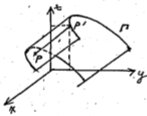
\includegraphics[ width=4 cm,height=2 cm]{b2p1-206-fig03-jpg}
 
  


    $\Gamma$: f$(x, y)$=0, z=0\hspace{40pt} g$(x, z)$=0 ,y=0\hspace{40pt} h$(y, z)$=0, X=0\\
    
    $\Delta$:\hspace{40pt}// $z$-axis \hspace{40pt}// $y$-axis\hspace{40pt}//$x$-axis\\
    
\par\indent
Let the directrix $\Gamma$ be on the $xy$-plane with equation $f ( x , y)$ = 0 , $z$ = 0 and direction $\Delta$ // $z$-axis.Then the equation  of this cylinder is


\begin{align*}
    $f(x, y)$ = 0 \hspace{16pt}(for \hspace{4pt}any \hspace{4pt}$z$ ). 
\end{align*}


\par
Similarly $g(x, z)$ = 0, and $h(y, z)$ = 0 are the equations of cylinders having directrices. on $xz$- and $yz$-planes and generatrices parallel to $y$- and $x$-axis. 


\par
These particular cylinders are \underline{right cylinders} since 
generatrices are perpendicular to the plane of the directrix.

\par
Observe that in cylindrical coordinates, $F(B, r) = 0$ represents a right cylinder with generatrix\hspace{4pt}//  $z$-axis. 

\par
G$(r \cos\theta, z)$ = $0$ represents a rihgt cylinder having directrix on the plane $\theta = 0$, and H$(r \sin\theta, z)$ = $0$ represents a right cylinder having directrix on the plane $\theta$$=$$\frac{\pi}{2}$

\par
 
 
\end{document}
